\documentclass[letterpaper,hyper]{THG_RFC}

% Fonts
\usepackage{ifluatex}
\ifluatex
  % Font
  \usepackage{luatextra, xunicode, unicode-math}
  \defaultfontfeatures{Ligatures=TeX}
  \setmainfont[
    UprightFont={*},
    BoldFont={* Bold},
    ItalicFont={* Italic},
    BoldItalicFont={* Bold Italic}
  ]{STIX}
  \setsansfont[
    UprightFont={*},
    BoldFont={* Bold},
    ItalicFont={* Italic},
    BoldItalicFont={* Bold Italic}
  ]{Source Sans Pro}
  \setmathfont[math-style=ISO, bold-style=ISO]{Latin Modern Math}
  \setmonofont[
    UprightFont={*},
    BoldFont={* Bold},
    ItalicFont={* Oblique},
    BoldItalicFont={* Bold Oblique}
  ]{DejaVu Sans Mono}
\else
  \usepackage{lmodern} % times / lmodern / mathpazo / palatino
  \usepackage[scaled=.95]{helvet}
  \usepackage{courier}
\fi

% Path to figures, plots
\graphicspath{{./pics/}{./plots/}}

%% TikZ
\usepackage{tikz}
\usetikzlibrary{patterns, shapes, shadows}

% Code snippets
\usepackage{listings}
\def\lstsetc{\lstset{language=C,
  numbers=left,
  xleftmargin=20pt,
  numberstyle=\tiny\color{gray},
  stepnumber=1,
  showspaces=false, 
  showstringspaces=false,
  breaklines=true,
  basicstyle=\footnotesize\ttfamily,
  stringstyle=\itshape,
  commentstyle=\itshape\bfseries,
  morekeywords={main, size_t, malloc, free,
    hsize_t, hid_t, herr_t, H5X_class_t, H5X_type_t,
    H5Fcreate, H5Fclose,
    H5Dcreate, H5Dopen, H5Dclose, H5Dwrite, H5Dread, H5Dquery,
    H5Qcreate, H5Qclose,
    H5Screate_simple, H5Sclose, H5Sget_select_npoints,
    H5Xcreate
    }
  }
}

% Title, author, etc
\title{Data Analysis Extensions}
\author{Jerome Soumagne}
\author{Quincey Koziol}
\date{July 17, 2014}
\rfcversion{2014-07-17.v1}
\revision{July 17, 2014}{Version 1 circulated for comment within The HDF Group.}

%% Start the document
\begin{document}

%% Title
\maketitle

%% Abstract
\begin{abstract}
Accessing and retrieving data from an HDF5 container can be a time consuming
process, particularly so when the data is very large. To enable,
ease and accelerate the process of querying data, we introduce in this RFC data
analysis extensions to query, select and index data.
\end{abstract}

\section{Introduction}
Data Analysis Extensions to the HDF5 API and data model can enable application
developers to create complex and high-performance queries on both metadata and
data elements within an HDF5 container and retrieve the results of applying
those query operations to an HDF5 container.
Support for data analysis operations on HDF5 containers can be defined via:
\begin{itemize}
\item New \textit{query} object\footnote{Query and view objects are
\textit{in-memory} objects, which therefore do not modify the content of the
container.\label{fn:object}} and API routines, enabling the construction of
query requests for execution on HDF5 containers;
\item New \textit{view} object\footref{fn:object} and API routines, which apply a query to an HDF5
container and return a set of references into the container that fulfills
the query criteria;
\item New \textit{index} object and API routines, which allows the creation of
indices on the contents of HDF5 containers, to improve query performance.
\end{itemize}

\section{Query Objects}
Query objects are the foundation of the data analysis operations in HDF5 and
can be built up from simple components in a programmatic way to create complex
operations using \textit{Boolean} operations. The core query API is composed of
two routines: \texttt{H5Qcreate} and \texttt{H5Qcombine}. \texttt{H5Qcreate}
creates new queries, by specifying an aspect of an HDF5 container, such as
data elements, link names, attribute names, etc., a match operator, such as
$=$, $\neq$, $\leq$, $\geq$, and a value for the match operator.
\texttt{H5Qcombine} combines two query objects into a
new query object, using Boolean operators such as $AND(\land)$ and $OR(\lor)$.
Queries created with \texttt{H5Qcombine} can be used as input to further
calls to \texttt{H5Qcombine}, creating more complex queries.

For example, a single call to \texttt{H5Qcreate} could create a query object
that would match data elements in any dataset within the container that are
equal to the value $17$. Another call to \texttt{H5Qcreate} could create a
query object that would match link names equal to $Pressure$.
Calling \texttt{H5Qcombine} with the $\land$ operator and those two query
objects would create a new query object that matched elements equal to $17$
in HDF5 datasets with link names equal to $Pressure$.
Creating the data analysis extensions to HDF5 using a \textit{programmatic
interface} for defining queries avoids defining a text-based query language
as a core component of the data analysis interface, and is more in keeping with
the design and level of abstraction of the HDF5 API.
The HDF5 data model is more complex than traditional database tables and a
simpler query model would likely not be able to express the kinds of queries
needed to extract the full set of components of an HDF5 container. A text-based
query language (or GUI) could certainly be built on top of the query API
defined here to provide a more user-friendly (as opposed to
\textit{developer-friendly}) query syntax like $Pressure = 17$. However, we
regard this as out-of-scope for now.

\todo{Add something about parallel queries / multi dataset serial}

\section{View Objects}
Applying a query to an HDF5 container creates an HDF5 view object. HDF5 view
objects are runtime, in-memory objects (i.e., not stored in a container) that
consist of read-only references into the contents of the HDF5 container that
the query was applied to. View objects are created with \texttt{H5Vcreate},
which applies a query to an HDF5 container, group hierarchy, or individual
object and produces the view object as a result. The attributes, objects,
and/or data elements referenced within a view can be retrieved by further API
calls.

For example, starting with the HDF5 container described in
\FigureRef{fig:HDF5File-Checkpoint}:

\begin{figure}
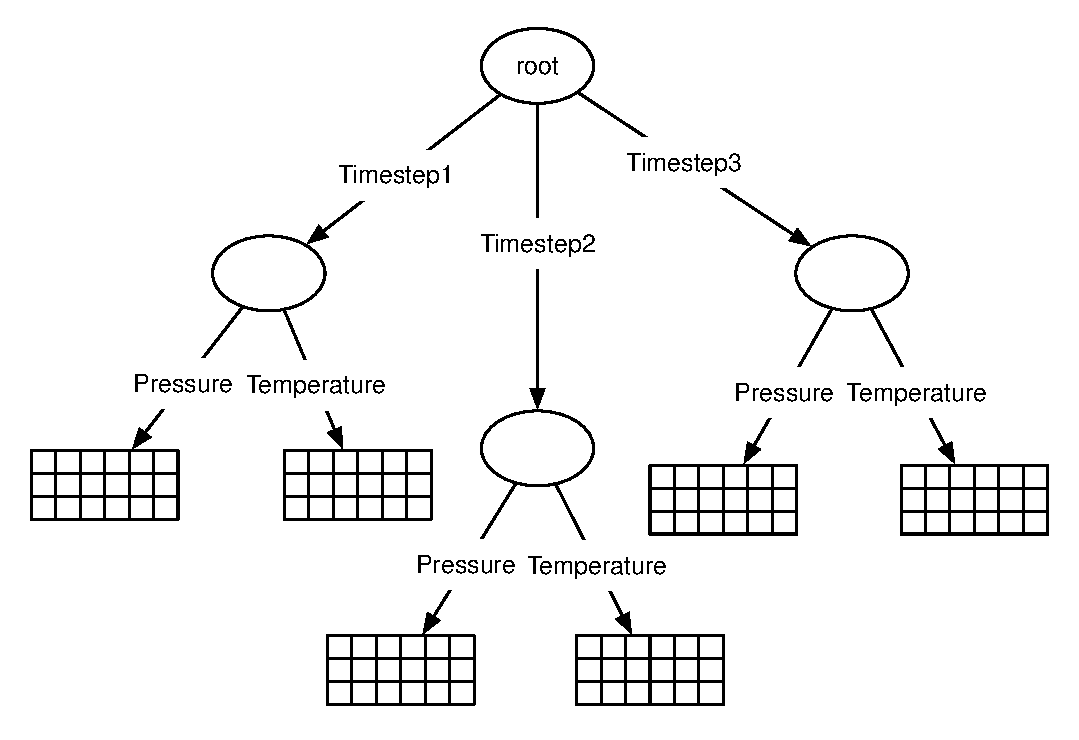
\includegraphics[width=\mediumfigwidth]{HDF5File-Checkpoint}
\caption{HDF5 container example.}
\label{fig:HDF5File-Checkpoint}
\end{figure}

Applying the $link\_name = Pressure$ query (described above) would result
in the view shown in \FigureRef{fig:HDF5File-Checkpoint-View1}, with the
underlying container grayed out and the view highlighted in green.

\begin{figure}
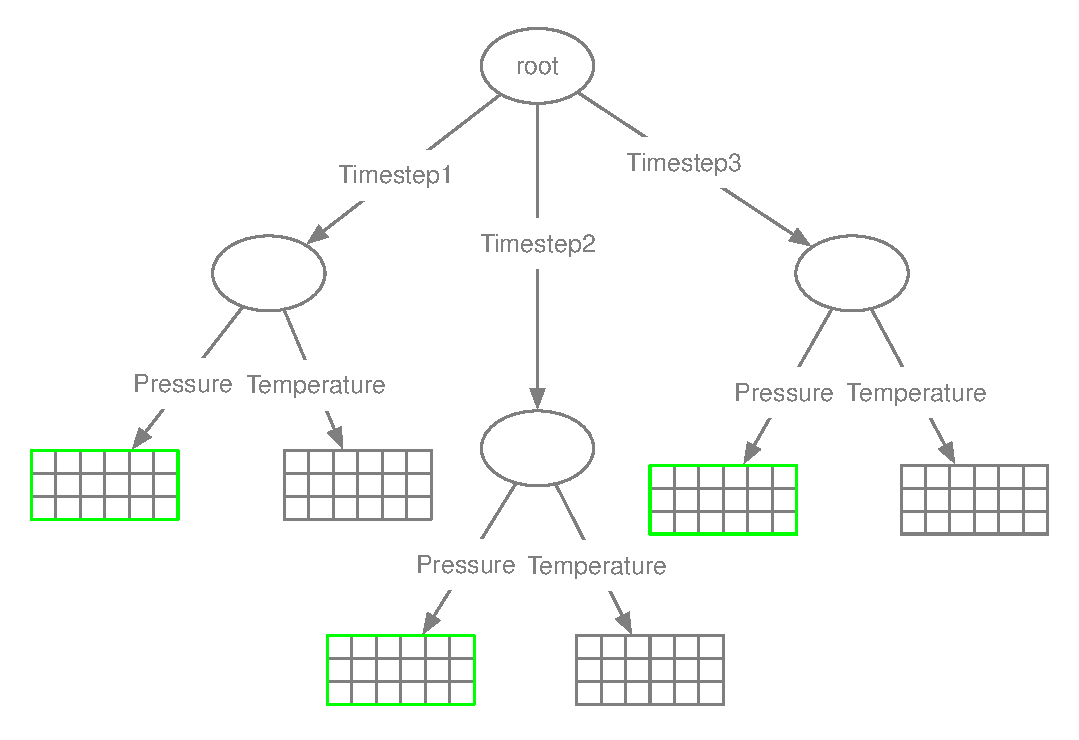
\includegraphics[width=\mediumfigwidth]{HDF5File-Checkpoint-View1}
\caption{HDF5 container example with query $link\_name = Pressure$ applied.}
\label{fig:HDF5File-Checkpoint-View1}
\end{figure}

Alternatively, applying the $data\_element = 17$ query (described above) would
result in the view shown in \FigureRef{fig:HDF5File-Checkpoint-View2}, with the
underlying container greyed out and the view highlighted in green.

\begin{figure}
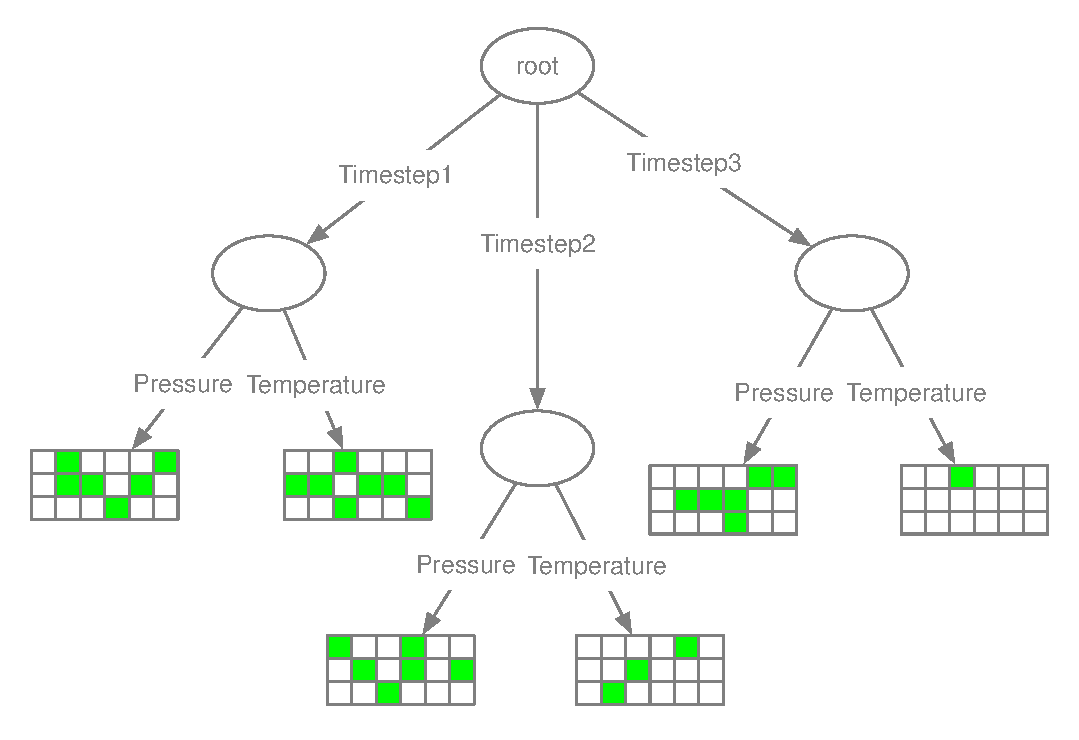
\includegraphics[width=\mediumfigwidth]{HDF5File-Checkpoint-View2}
\caption{HDF5 container example with query $data\_element = 17$ applied.}
\label{fig:HDF5File-Checkpoint-View2}
\end{figure}

Finally, applying the combined $(link\_name = Pressure)\land(data\_element = 17)$
query (described above) would result in the view shown in
\FigureRef{fig:HDF5File-Checkpoint-View3}, with the underlying container
greyed out and the view highlighted in green.

\begin{figure}
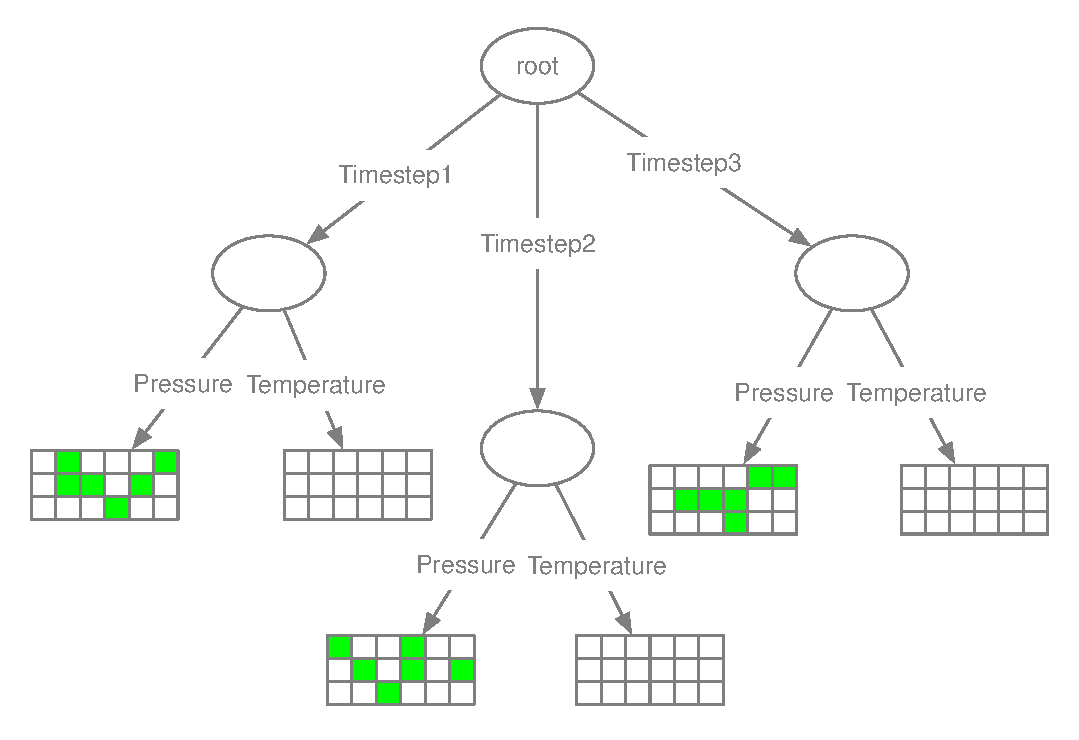
\includegraphics[width=\mediumfigwidth]{HDF5File-Checkpoint-View3}
\caption{HDF5 container example with query $(link\_name = Pressure)\land(data\_element = 17)$ applied.}
\label{fig:HDF5File-Checkpoint-View3}
\end{figure}

Views can be thought of as containing a set of HDF5 references (object,
dataset region or attribute references) to components of the underlying
container, retaining the context of the original container. For example, the
view containing the results of the $(link\_name = Pressure)\land(data\_element = 17)$
query will contain three dataset region references, which
can be retrieved from the view object and probed for the dataset and selection
containing the elements that match the query with the existing \texttt{H5Rdereference}
and \texttt{H5Rget\_region} API calls. Note that selections returned from a region
reference retain the underlying dataset's dimensionality and coordinates---they
are not \textit{flattened} into a 1-D series of elements. The selection returned
from a region reference can also be applied to a different dataset in the container,
allowing a query on pressure values to be used to extract temperature values,
for example.

\section{Index Objects}
The final component of the data analysis extensions to HDF5 is the index object.
Index objects are designed to accelerate creation of view objects from
frequently occurring query operations.
For example, if the $(link\_name = Pressure)\land(data\_element = 17)$ query
(described above) is going to be frequently executed on the container, indices
could be created in that container, which would speed up the creation of views
when querying for link names and for data element values. Indices created for
accelerating the $link\_name = Pressure$ or $data\_element = 17$ queries
would also improve view creation for the more complex
$(link\_name = Pressure)\land(data\_element = 17)$ query.

Although creating indices for metadata components of queries, such as link or
attribute names, is possible, we focus on index creation for
dataset elements, as they represent the largest volume of data in typical HPC
application usage of HDF5. Queries with metadata components execute properly,
\todo{Must write about metadata indexing} but are not able to be accelerated
with an index currently.

The indexing API works in conjunction with the view API. When an \texttt{H5Vcreate}
call is made for a group or dataset, an index attached to any dataset queried
for element value ranges will be used to speed up the query process and return
a dataspace selection to the library for later use.

There are different techniques for creating data element indices, and the most
efficient method will vary depending on the type of the data that is to be
indexed, its layout, etc. We therefore define a new interface for the HDF5
library that uses a plugin mechanism.

\subsection{Indexing Interface and Plugins}

A new HDF5 interface is defined for adding third-party indexing plugins,
such as FastBit~\cite{Wu05}, ALACRITY~\cite{alacrity13}, etc.
The interface provides indexing plugins with efficient access to the contents of
the container for both the creation and the maintenance of indices. In addition,
the interface allows third-party plugins to create private data structures
within the container for storing the contents of the index.

Index objects are stored in the HDF5 container that they apply to, but are not
visible in the container's group hierarchy\footnote{Plugin developers, note that
the HDF5 library's existing anonymous dataset and group creation calls can be
used to create objects in HDF5 files that are not visible in the container's
group hierarchy.}.
Instead, index objects are part of the metadata for the file itself. New index
objects are created by passing an H5 container to be indexed and the index
plugin ID to the \texttt{H5Xcreate} call.
Index information (such as plugin id and index metadata) is stored at index
creation time\footnote{This therefore introduces a file format change},
and when the user later calls \texttt{H5Dopen}, the plugin open
callback will retrieve this stored information and make use of the corresponding
index plugin for all subsequent operations. Similarly, calling \texttt{H5Dclose}
will call the plugin index close callback and close the objects used to store
the index data.

\begin{figure}
\tikzstyle{textBox}    = [rectangle, text centered, font=\small \bfseries]
\tikzstyle{appBox}     = [draw, rectangle, rounded corners, fill=white, dashed, very thick]
\tikzstyle{fileBox}    = [draw, rectangle, fill=white, drop shadow={opacity=0.25}]
\tikzstyle{headerBox}  = [draw, rectangle, fill=rulecolor, font=\footnotesize]
\tikzstyle{dataBox}    = [draw, rectangle, thick, fill=white, pattern color=rulecolor, pattern=dots, font=\small]
\tikzstyle{cacheBox}   = [draw, rectangle, thick, fill=black!10, drop shadow={opacity=0.25}]
\tikzstyle{cacheBoxes} = [draw, tape, tape bend top=none, fill=rulecolor, double copy shadow]

%\tikzstyle{trans} = [->, >=stealth, thick, text centered, font=\footnotesize]
\tikzstyle{message} = [draw=blue, ->, very thick, shorten <=2pt, shorten >=2pt, 
  text centered, text width=2.5cm, font=\footnotesize]

\begin{tikzpicture}

\node[appBox, minimum height=4cm, minimum width=14cm] (app) {};
\node[textBox, minimum height=1cm, minimum width=2cm, below left=2mm of app.north east] (apptitle) {Application memory};
\node[cacheBox, minimum height=3.6cm, minimum width=6.4cm, right=2mm of app.west] (cache) {};
\node[rectangle, minimum height=3.6cm, minimum width=2.9cm, right=2mm of cache.west] (cachecol1) {};
\node[rectangle, minimum height=3.6cm, minimum width=2.9cm, right=2mm of cachecol1.east] (cachecol2) {};
\node[headerBox, minimum width=2.5cm, minimum height=0.7cm, below=1.7mm of cachecol1.north] (cache1) {Dataset header};
\node[headerBox, minimum width=2.5cm, below=-1pt of cache1] (cache2) {\dots};
\node[headerBox, minimum width=2.5cm, below=-1pt of cache2] (cache3) {Datatype};
\node[headerBox, minimum width=2.5cm, below=-1pt of cache3] (cache4) {Dataspace};
\node[headerBox, minimum width=2.5cm, below=-1pt of cache4] (cache5) {\dots};
\node[headerBox, minimum width=2.5cm, below=-1pt of cache5] (cache6) {Attributes};
\node[headerBox, minimum width=2.5cm, below=-1pt of cache6] (cache7) {\dots};

\node[textBox, minimum height=1cm, minimum width=2cm, below=1mm of cachecol2.north] (cachetitle) {Metadata cache};
\node[cacheBoxes, below=1.5cm of cachecol2.north, minimum width=2cm, minimum height=1cm] () {};

\node[fileBox, minimum height=1cm, minimum width=14cm, below=5mm of app] (file) {};
\node[textBox, minimum height=1cm, minimum width=2cm, right=4mm of file.west] (filetitle) {File};
\node[headerBox, thick, minimum height=1cm, minimum width=1cm, right=1.5cm of filetitle] (fileheader) {};
\node[dataBox, minimum height=1cm, minimum width=5cm, right=3cm of fileheader] (filedata) {Dataset data};

\node[rectangle, fill=white, minimum height=1cm, minimum width=5cm, above=2cm of filedata, drop shadow={opacity=0.25}] () {};
\node[dataBox, minimum height=1cm, minimum width=5cm, above=2cm of filedata] (appdata) {Dataset data};

\draw[message] (cache7.east) -| (fileheader.north);
\draw[message] (appdata.south west) -- (filedata.north west);
\draw[message] (appdata.south east) -- (filedata.north east);

\end{tikzpicture}

\caption{HDF5 stores multidimensional arrays (datasets)
  along with metadata in a file. In this case, a dataset is contiguously mapped
  from the application memory to a file, its data structure being described in
  the metadata cache.}
\label{fig:hdf5filestruc}
\end{figure}

When a call to \texttt{H5Dwrite} is made, the index plugin \texttt{pre\_update} and
\texttt{post\_update} callbacks will be triggered, allowing efficient index
update by first telling the index plugin the region that is going to be updated
with new data, and then realizing the actual index update, after the dataset
write has completed. This allows various optimization to be made, depending on
the data selection passed and the index plugin used. For example, a plugin could
store the region and defer the actual index update until the dataset is closed,
hence saving repeated index computation/update calls.

When a call to \texttt{H5Vcreate} is made, the index plugin query callback will be
invoked to create a selection of elements in the dataset that match the query
parameters. Applications can also use the new \texttt{H5Dquery} routine to directly
execute a query on a dataset (accelerated by any index defined on the dataset),
retrieving the selection within that dataset that matches the query.

Because the amount of space taken by the index cannot be directly retrieved by
the user since the datasets storing the indices should be \textit{anonymous}
and not visible from the file hierarchy, we also plan on adding callbacks to
query from a specified dataset the amount of space the index that is attached
to it takes.

\subsubsection{Interface}

{\lstsetc
\begin{lstlisting}
typedef struct {
    unsigned version;     /* Version number of the index plugin class struct */
                          /* (Should always be set to H5X_CLASS_VERSION, which
                           *  may vary between releases of HDF5 library) */
    unsigned id;          /* Index ID (assigned by The HDF Group, for now) */
    const char *idx_name; /* Index name (for debugging only, currently) */
    H5X_type_t type;      /* Type of data indexed by this plugin */

    /* Callbacks, described above */
    void *(*create)(hid_t file_id, hid_t dataset_id, hid_t xcpl_id,
        hid_t xapl_id, size_t *metadata_size, void **metadata);
    herr_t (*remove)(hid_t file_id, hid_t dataset_id, size_t metadata_size,
        void *metadata);
    void *(*open)(hid_t file_id, hid_t dataset_id, hid_t xapl_id,
        size_t metadata_size, void *metadata);
    herr_t (*close)(void *idx_handle);
    herr_t (*pre_update)(void *idx_handle, hid_t dataspace_id, hid_t xxpl_id);
    herr_t (*post_update)(void *idx_handle, const void *buf, hid_t dataspace_id,
            hid_t xxpl_id);
    herr_t (*query)(void *idx_handle, hid_t query_id, hid_t xxpl_id,
        hid_t *dataspace_id);
    herr_t (*refresh)(void *idx_handle, size_t *metadata_size, void **metadata);
} H5X_class_t;
\end{lstlisting}
}

\subsubsection{Current and future plugins}

Current implementations for FastBit and ALACRITY index packages are already
present, as well as a brute force indexing plugin. In the future more plugins
will be added, with and without external dependency.
To satisfy that need, dynamic plugin loading and registration will be supported,
allowing external libraries to plug to the current interface.
\todo{pytable indexing?}

\subsection{Limitations}

There are some existing limitations in the use of indices in the current
implementation: FastBit and
ALACRITY do not support incremental updates, an index is a shared resource for
a dataset. Taken together, these conspire to put limits on application updates
to datasets with indices.
Additionally, because FastBit and Alacrity don't allow incremental updates to
an index, each modification to an existing index forces the index to be entirely
rebuilt. The limitation in FastBit and Alacrity will need to be addressed in
the base packages' implementation, so that they can make incremental updates
to their index information.

\subsubsection*{Questions}
Some questions are still open regarding the handling on indices:
\begin{itemize}
\item How could an index be built in parallel for a dataset that already exists?
\item How to handle index updates when the specified index plugin is not available?
(In traditional databases, stored procedures are saved with the data and
therefore available at any time, but that is not the case here)
\item How to handle index queries when the specified index plugin is not
available?
\end{itemize}

\section{HDF5 and tools}

Existing HDF5 tools must be compatible and take into account the existence of
indices in the file if there are any. For reference, the following behavior for
the tools is given:

\begin{itemize}
\item h5dump: report index information
\item h5ls: report index information
\item h5diff: ignore index information?
\item h5repack: copy index information
\item h5edit: ignore index information?
\item h5toh4: ignore index information?
\item h5import: copy index information
\end{itemize}

\section{Usage Example}

In the following example, we show how one can make use of the query and
indexing interface to get a dataspace selection within a dataset,
for simplicity we first create a dataset within the file, then open it to
create and attach a new index, to finally query data from it.

{\lstsetc
\begin{lstlisting}
#define NTUPLES 256

int
main(int argc, char *argv[])
{
    float data[NTUPLES];
    hsize_t dims[1] = {NTUPLES};
    hid_t t file_id, dataspace_id, dataset_id;
    hid_t query_id, result_space_id;
    size_t result_npoints;
    float *result;
    int i;

    /* Initialize data. */
    for(i = 0; i < NTUPLES; i++) data[i] = (float) i;

    /* Create file. */
    file_id = H5Fcreate(file_name, H5F_ACC_TRUNC, H5P_DEFAULT, H5P_DEFAULT);

    /* Create the data space for the dataset. */
    dataspace_id = H5Screate_simple(rank, dims, NULL);

    /* Create dataset. */
    dataset_id = H5Dcreate(file_id, "Pressure", H5T_NATIVE_FLOAT, dataspace_id,
        H5P_DEFAULT, H5P_DEFAULT, H5P_DEFAULT);

    /* Write dataset. */
    H5Dwrite(dataset_id, H5T_NATIVE_FLOAT, H5S_ALL, H5S_ALL, H5P_DEFAULT, data);

    /* Close the dataset. */
    H5Dclose(dataset_id);

    /* Close dataspace. */
    H5Sclose(dataspace_id);

    /* Open dataset. */
    dataset_id = H5Dopen(file_id, "Pressure", H5P_DEFAULT);

    /* Create index using FastBit. */
    H5Xcreate(file_id, H5X_PLUGIN_FASTBIT, dataset_id, H5P_DEFAULT);

    /* Close the dataset. */
    H5Dclose(dataset_id);

    /* Create a simple query */
    query_id = H5Qcreate(H5Q_TYPE_DATA_ELEM, H5Q_MATCH_EQUAL, H5T_NATIVE_FLOAT,
        &query_value);

    /* Open dataset. */
    dataset_id = H5Dopen(file_id, "Pressure", H5P_DEFAULT);

    /* Use query to select elements in the dataset. */
    result_space_id = H5Dquery(dataset_id, query_id);

    /* Allocate space to read data. */ 
    result_npoints = (size_t) H5Sget_select_npoints(result_space_id);
    result = malloc(result_npoints * sizeof(float));

    /* Read data using result_space_id. */
    H5Dread(dataset_id, H5T_NATIVE_FLOAT, H5S_ALL, result_space_id,
        H5P_DEFAULT, result);

    /* Use result. */

    /* Free result. */
    free(result);

    /* Close the dataset. */
    H5Dclose(dataset_id);

    /* Close dataspace. */
    H5Sclose(result_space_id);

    /* Close query. */
    H5Qclose(query_id);

    /* Close the file. */
    H5Fclose(file_id);
}
\end{lstlisting}
}

\section{Conclusion}

%% Close
\section*{Revision History}
\makerevisions

%% References
\bibliographystyle{ieeetr}
\bibliography{analysis_ext}

\end{document}
